
\documentclass{article}
\usepackage[headheight=20pt, margin=1.0in, top=1.2in]{geometry}
\usepackage{amsmath, amssymb, amsthm, thmtools, tcolorbox, array, graphicx, makeidx, cancel, multirow, fancyhdr, xypic, color, nicefrac, rotating, multicol, caption, subcaption, xcolor, tikz, tikz-3dplot, tikz-cd, pgfplots, import, enumitem, calc, booktabs, wrapfig, siunitx, hyperref,float}
\hypersetup{colorlinks=true,linkcolor=blue}
\usepackage[all]{xy}
\usepackage{esint}
\setlength{\parindent}{0in}
\sisetup{per-mode = symbol}
\usetikzlibrary{calc,arrows,svg.path,decorations.markings,patterns,matrix,3d,fit}
\usepgfplotslibrary{groupplots}
\pgfplotsset{compat=newest}
\newtcolorbox{mydefbox}[2][]{colback=red!5!white,colframe=red!75!black,fonttitle=\bfseries,title=#2,#1}
\newtcolorbox{mythmbox}[2][]{colback=gray!5!white,colframe=gray!75!black,fonttitle=\bfseries,title=#2,#1}
\newtcolorbox{myexamplebox}[2][]{colback=green!5!white,colframe=green!75!black,fonttitle=\bfseries,title=#2,#1}
\newtcolorbox{mypropbox}[2][]{colback=blue!5!white,colframe=blue!75!black,fonttitle=\bfseries,title=#2,#1}
\declaretheoremstyle[headfont=\color{blue}\normalfont\bfseries,]{colored}
\theoremstyle{definition}
\newtheorem{theorem}{Theorem}
\newtheorem{corollary}[theorem]{Corollary}
\newtheorem{lemma}[theorem]{Lemma}
\newtheorem{proposition}[theorem]{Proposition}
\newtheorem{problem}[theorem]{Problem}
\newtheorem{definition}[theorem]{Definition}
\newtheorem{exercise}[theorem]{Exercise}
\newtheorem{example}[theorem]{Example}
\newtheorem{solution}[theorem]{Solution}
\newtheorem*{thm}{Theorem}
\newtheorem*{lem}{Lemma}
\newtheorem*{prob}{Problem}
\newtheorem*{exer}{Exercise}
\newtheorem*{prop}{Proposition}
\def\R{\mathbb{R}}
\def\F{\mathbb{F}}
\def\Q{\mathbb{Q}}
\def\C{\mathbb{C}}
\def\N{\mathbb{N}}
\def\Z{\mathbb{Z}}
\def\Ra{\Rightarrow}
\def\e{\epsilon}
\newcommand{\typo}[1]{{\color{red}{#1}}}
\newcommand\thedate{\today}
\newcommand{\mb}{\textbf}
\newcommand{\norm}[2]{\|{#1}\|_{#2}}
\newcommand{\normm}[1]{\|#1\|}
\newcommand{\mat}[1]{\begin{bmatrix} #1 \end{bmatrix}}
\newcommand{\eqtext}[1]{\hspace{3mm} \text{#1} \hspace{3mm}}
\newcommand{\set}[1]{\{#1\}}
\newcommand{\inte}{\textrm{int}}
\newcommand{\ra}{\rightarrow}
\newcommand{\minv}{^{-1}}
\newcommand{\tx}[1]{\text{ {#1} }}
\newcommand{\abs}[1]{|#1|}
\newcommand{\mc}[1]{\mathcal{#1}}
\newcommand{\uniflim}{\mathop{\mathrm{unif\lim}}}
\newcommand{\notimplies}{\mathrel{{\ooalign{\hidewidth$\not\phantom{=}$\hidewidth\cr$\implies$}}}}
\pagestyle{fancy}
\fancyhf{}
\fancyhead[L]{Title of the Document}
\fancyhead[C]{}
\fancyhead[R]{\thepage}
\fancyfoot[L]{}
\fancyfoot[C]{}
\fancyfoot[R]{}
\renewcommand{\headrulewidth}{0.4pt}
\renewcommand{\footrulewidth}{0.4pt}
\numberwithin{equation}{section}
% Increase spacing between paragraphs
\setlength{\parskip}{1em}
% Increase spacing before and after sections
\usepackage{titlesec}
\titlespacing*{\section}{0pt}{3ex plus 1ex minus .2ex}{2ex plus .2ex}
\titlespacing*{\subsection}{0pt}{2ex plus 1ex minus .2ex}{1ex plus .2ex}
\titlespacing*{\subsubsection}{0pt}{1ex plus 1ex minus .2ex}{1ex plus .2ex}
\title{\textbf{Title of the Document}}
\author{Author Name}
\date{\today}
\begin{document}
\maketitle
\tableofcontents
\newpage
\section{Exercises}
\begin{enumerate}
    \item Let $(X,d)$ be a metric space and $S \subseteq X$. Show that $\overline{S}^{int} = \varnothing$.
    \item Show that for an arbitrary choice of $a,b,r \in \mathbb{R}$, the closed disk $E = \{(x,y) \ | \ (x-a)^2 + (y-b)^2 \leq r^2\}$ is a bounded set in $\mathbb{R}^2$.
    \item Let $f: X \to \mathbb{R}$ be a metric space and for $x,y \in X$. Show that if $d(x,y) < \varepsilon$ for every $\varepsilon > 0$, then $x = y$.
\end{enumerate}

\begin{proof}[Exercise 2.1]
(i) Assume $\overline{S}^{int} \neq \varnothing$. Then $\exists x \in \overline{S}^{int}, \exists r > 0$ such that $B_r(x) \subseteq S^{int}$. However, by $x \notin S$, this value of $r > 0$ implies $B_r(x) \cap S^c \neq \varnothing \Rightarrow B_r(x) \nsubseteq S$, which is a contradiction. Hence, $x \notin S \Rightarrow S^{int} = \varnothing$.
\end{proof}

\begin{proof}[Exercise 2.2]
(ii) A set $S$ is bounded iff $\exists M \in \mathbb{R}^+ \ \forall x, y \in S \ d(x, y) \leq M$. Let $a, b, r \in \mathbb{R}$. So $E = \{(x, y) \in \mathbb{R}^2 \ | \ (x-a)^2 + (y-b)^2 \leq r^2\}$. 
\begin{align*}
&\Rightarrow x^2 - 2ax + a^2 + y^2 - 2yb + b^2 \leq r^2 \\
&\Rightarrow x^2 - 2ax + y^2 - 2yb \leq r^2 - a^2 - b^2 \\
&\Rightarrow x^2 + y^2 \leq r^2 - a^2 - b^2 + 2ax + 2yb
\end{align*}
We need to show $x^2$ is bounded.
\begin{align*}
&(x-a)^2 \leq r^2 \\
&\Rightarrow |x-a| \leq |r| \\
&\Rightarrow |x-a| + a \leq |r| + |a| \\
&\Rightarrow |x| \leq |x-a| + a \leq |x-a| + |a| \leq R + |a|
\end{align*}
Thus $x^2$ is bounded.
\end{proof}

\Rightarrow |y| \leq r + |a| 
\Rightarrow x^2 \leq (r + |a|)^2
$
Same for \(y_i\):
$
y_i^2 \leq (r + |b|)^2
$
$
\forall z = (x,y) \in D_{r,(a,b)}
$
$
\|z\| = \sqrt{x^2 + y^2} \leq \sqrt{(r + |a|)^2 + (r + |b|)^2}
$
Thus if \(M = \sqrt{(r + |a|)^2 + (r + |b|)^2}\), the bond holds.

\# 15 named boundedness \(=\) distance boundedness.

Let \(x = (x_1,x_2), y = (y_1,y_2) \in D_{r,a,b}\)

$
z_i \in \{x_i,y_i\}
$
$
(x_2 - a)^2 + (y_2 - b)^2 = r^2 
\Rightarrow d(z_i, (a,b)) = \sqrt{(x_2 - a)^2 + (y_2 - b)^2} \leq r
$
$
\Rightarrow d(x,y) \leq d(x_1,(a,b)) + d(y_1,(a,b))
$
$
= \sqrt{(x_1 - a)^2 + (x_1 - b)^2} + \sqrt{(y_1 - a)^2 + (y_1 - b)^2}
$
$
\leq r + r = 2r
$

\begin{itemize}
    \item[(iii)] Suppose that $x \neq y$. Then $d(x, y) \ne 0$. Thus if we choose $\epsilon = d(x, y) \implies \epsilon > 0$ but $d(x, y) \ge \epsilon$ (contradiction).

    \item[(contradiction)] Suppose $ x \neq y $ and so $ d(x, y) \neq 0 $. 

    Choose $\epsilon > 0$ so that $\epsilon = \frac{d(x,y)}{2}$. Then we must have $d(x, y) < \epsilon = \frac{d(x, y)}{2}$, which is a contradiction, as this implies if $d(x, y) \leq \frac{d(x, y)}{2} \implies d(x, y) = \epsilon = \frac{d(x, y)}{2}$

    $ \implies d(x, y) = \frac{d(x, y)}{2} $
    $ \implies 2\epsilon \leq \epsilon $

    Thus, $x = y$.

    \item[(iv)] Let $(V, \|.\|)$ be a normed vsp. Then let $r > 0$ and $x \in V$. Then
    $ B_{r}(x) = \{y \in V | d(x, y) < r \} $
    $ B_{\epsilon + r} (0) = \{y \in V | d(0, y) < r + \| x \| \} $

    $
    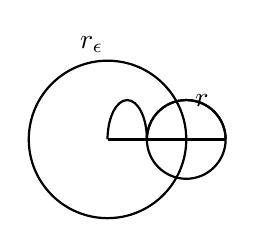
\begin{tikzpicture}
        \draw [thick] (0,0) circle [radius=1];
        \draw [thick] (1,0) circle [radius=0.5];
        \draw [thick] (0,0) -- (1,0);
        \draw [thick] (1,0) -- (1.5,0);
        \draw [thick] (1.5,0) arc [start angle=0, end angle=180, radius=0.5];
        \draw [thick] (0.5,0) arc [start angle=0, end angle=180, x radius=0.25, y radius=0.5];
        \node at (-0.2, 1.2) {$r_\epsilon$};
        \node at (1.2, 0.5) {$r$};
    \end{tikzpicture}
    $

    Let $y \in B_{r}(x)$. 
    $d(0, y) \leq d(0, x) + d(x, y)$
    $\leq \| x \| + r $
    $ \implies B_{r}(x) \leq B_{\epsilon + r} (0) $

    \item[(v)] Suppose $\mathcal{S}$ is bounded. Then $\exists M \in \mathbb{R}$ such that $\forall x \in \mathcal{S} \| x \| \leq M$. (Equivalent to $\exists M \in \mathbb{R}: \forall x \in \mathcal{S} x \in B_{M}(0)$
\end{itemize}\end{document}